%
% File acl2020.tex
%
%% Based on the style files for ACL 2020, which were
%% Based on the style files for ACL 2018, NAACL 2018/19, which were
%% Based on the style files for ACL-2015, with some improvements
%%  taken from the NAACL-2016 style
%% Based on the style files for ACL-2014, which were, in turn,
%% based on ACL-2013, ACL-2012, ACL-2011, ACL-2010, ACL-IJCNLP-2009,
%% EACL-2009, IJCNLP-2008...
%% Based on the style files for EACL 2006 by 
%%e.agirre@ehu.es or Sergi.Balari@uab.es
%% and that of ACL 08 by Joakim Nivre and Noah Smith

\documentclass[11pt,a4paper]{article}
\usepackage[hyperref]{acl2020}
\usepackage{times}
\usepackage{latexsym}
\usepackage{graphicx}
\renewcommand{\UrlFont}{\ttfamily\small}

% This is not strictly necessary, and may be commented out,
% but it will improve the layout of the manuscript,
% and will typically save some space.
\usepackage{microtype}

\aclfinalcopy % Uncomment this line for the final submission
%\def\aclpaperid{***} %  Enter the acl Paper ID here

%\setlength\titlebox{5cm}
% You can expand the titlebox if you need extra space
% to show all the authors. Please do not make the titlebox
% smaller than 5cm (the original size); we will check this
% in the camera-ready version and ask you to change it back.

\newcommand\BibTeX{B\textsc{ib}\TeX}

\title{Team 24 Final Report}

\author{Max Hamilton \\
  \texttt{johnmaxh@umich.edu} \\\And
  Gaurav Kaul \\
  \texttt{kaulg@umich.edu} \\\And
  Zack Zhang \\
  \texttt{zacklt@umich.edu} \\}

\begin{document}
\maketitle

\begin{abstract}
There are many exciting benchmarks in the field of NLP where human performance far exceeds current models. In this report we focus on CommonsenseQA, Conversational Entailment, and Everyday Actions in Text (EAT) and present our solutions to these three tasks. Our solutions utilize automated hyperparameter search, specialized data preprocessing, and a custom loss function. We believe that the models we trained are competitive with other groups. Finally, our team has learned many lessons including tuning strategies, validation techniques, and the power of pretrained transformer based models.
\end{abstract}
\section{Introduction}
CommonsenseQA \citep{talmor2019commonsenseqa}, which focuses on inference of answers through implicit common sense, was developed as a dataset that machine learning models could not easily learn through simple memorization of the input texts. At the time of the publication, the best baseline is based on BERT-large \citep{devlin2019bert} and obtains 56\% accuracy, well below human performance, which is 89\% (Talmor et al., 2018). This is unsurprising since Bert-large was the general state-of-the-art model at that time and is still one of the most popular baseline models. A common problem is that researchers often compare untuned bert models with fine-tuned models like GPT-2 \citep{radford2019language} and ALBERT \citep{lan2020albert}. Thus, we hypothesize that after reimplementation of the original model, more explicit hyperparameter turning might be helpful in showing a more realistic baseline.

For the Conversational Entailment \citep{zhang-chai-2010-towards} task, the model is given a conversation and a hypothesis, and is tasked with deciding whether the hypothesis can be concluded from the conversation. This makes the conversational entailment task a binary classification problem. In addition, the input size is variable and the data set (we were provided) is relatively small, with roughly 500 examples for training. This suggests that overfitting could be an issue.

The EAT dataset also presents interesting challenges. For each story composed of multiple sentences, we need to first detect if that story makes sense, and if not, which sentence the story first stops making sense. We can view this as two separate tasks: a binary plausibility prediction over the entire story and a breakpoint classification over all the sentences. As an extra challenge, the number of sentences in each story can vary, so the number of classes to predict over changes dynamically per sample. There is also missing information in breakpoints labels, as only the first sentence that stops making sense is provided, but not the reason that sentence does not make sense or which prior sentences it contradicts with. 


\section{Computational Models}

\subsection{CommonsenseQA}
Since the original test data is withheld by the creators for the leaderboard, we have taken the same proportion of data out of the training data as our validation data and used the original validation data as the test data. We have a roughly 8:1:1 ratio among the train, validation, and test datasets. We used “random split” as the authors have found it harder than (lower accuracies) their question-concept split. For embeddings, wordpieces are trained separately, such that the most frequent words remain together and the less frequent words get split eventually down to characters. For our activation function we used Gaussian Error Linear Units \citep{hendrycks2020gaussian}. When deciding our model architecture, We adapted BERT for choosing an answer among multiple candidates. A detailed description of the bert model can be found in the original paper. On top of the final layer of BERT, we pool the output, add a dropout regularizer, add a linear layer, and finally a softmax upon the results of all the 5 choices to select the best answer. We have decided to tune the following hyperparameters (below are the initial random coarse search ranges)

\begin{itemize}
    \item learning rate:  1e-6, 1e-4
    \item batch size:  48, 32, 8 
    \item max sequence length:  80, 48
    \item hidden dropout probability:  0.1, 0.2
    \item hidden activation:  gelu
    \item architecture: BERT
    \item tokenizer: BertTokenizer
    \item model:  BertForMultipleChoice
    \item pretrained model name: bert-base-uncased
\end{itemize}

For the optimizer we used AdamW. The coefficients used for computing running averages of gradient and its square are 0.9 and 0.999, the term added to the denominator to improve numerical stability is 1e-8, and the weight decay coefficient is 1e-2.

Then we performed fine-tuning upon the best result above using the ray tune library \citep{liaw2018tune} to obtain the best hyperparameters.



\subsection{Conversational Entailment}

\begin{figure}[t]
    \centering
    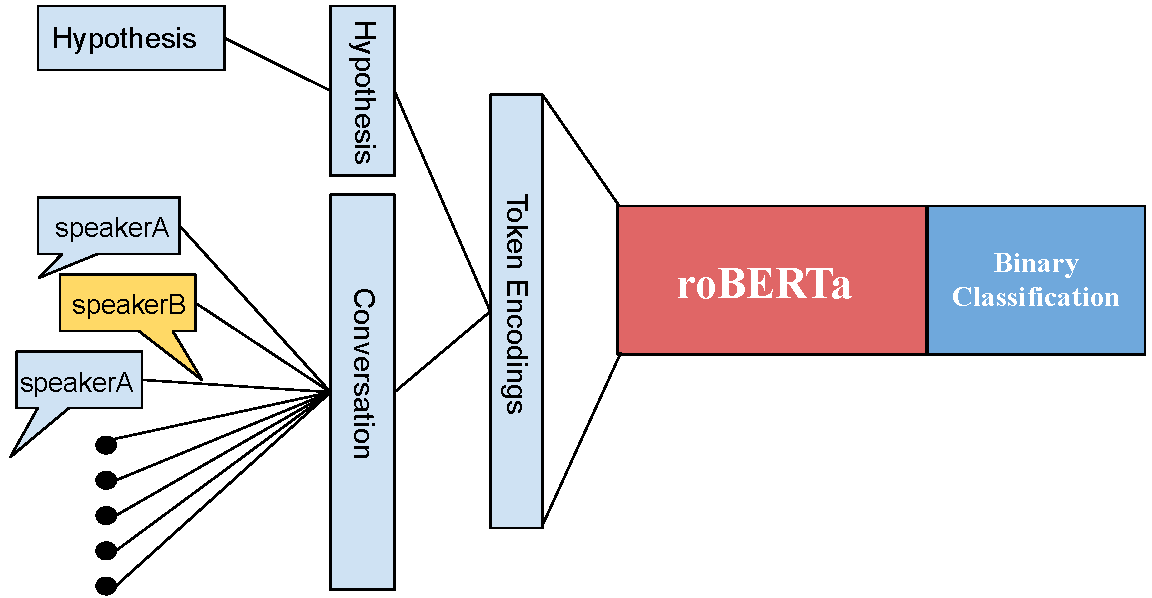
\includegraphics[width=\linewidth]{assets/ce_diagram.pdf}
    \caption{Overview of the Conversational Entailment Task architecture. Conversation-Hypothesis sequence pairs are encoded and fed into roBERTa, which get converted into attention embedding.Theese embeddings are then used to classify entailment via a binary classification head}
\end{figure}

When working with the Conversational entailment dataset, there were very obvious problems that made it difficult to pinpoint an obvious model choice. The benchmark paper we were given utilized a statistical approach \citep{zhang-chai-2009-know}. But later down the line it became more apparent that this might be too complex to implement in our time frame. 

A big problem that we needed to address in our computational model was variable length input with a fixed size output. Essentially our choice of model needed to be able to handle variable length conversations and output a fixed binary classification decision.This problem made us initially look at some form of a recurrent neural net, with a many to one format with an input of conversation and hypothesis, and output  of a binary decision. This seemed like a good idea at first but a more recent trend has highlighted that attention based models \citep{vaswani2017attention} can outperform Recurrent neural networks in most benchmark tasks. So after looking at potential models to use we ended up exploring transformers. Our initial tests were with BERT and roBERTa \citep{liu2019roberta} models. 
    
Our Transformer based approach was very effective since it initially gave us an accuracy much higher than the random guessing, which was a good start. We tested many different versions of BERT and roBERTa: the base, large, and MNLI \citep{N18-1101} pretrained versions. We ended up finding that our best results were with roBERTa large pre-trained(MNLI). We used the Pytorch encoder for sequence pairs and put our hypothesis as our classification sequence followed by the conversation. We then gave it a binary classification head in order to output true or false for the entailment prediction.

When pre-processing our input for the conversation we needed to take into account that the model won't know who's speaking during the conversation sequence, so during pre-processing we included “speakerB says” and “speakerA says” before the speaker spoke to function as separation tokens that help the model make the decision when the hypothesis mentions “speakerB”/ “speakerA”.

\subsection{EAT}

\begin{figure}[t]
    \centering
    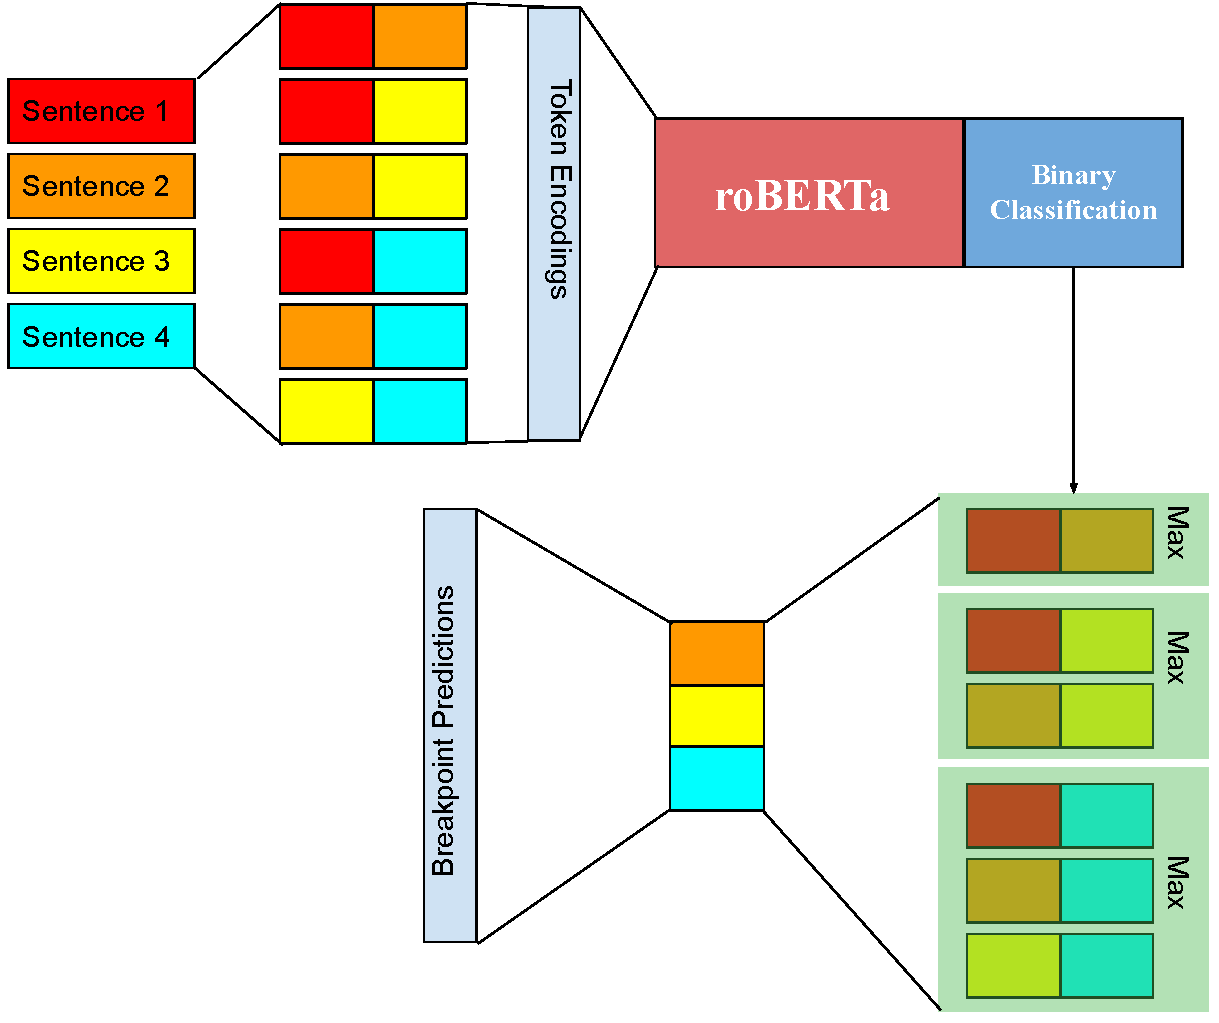
\includegraphics[width=\linewidth]{assets/eat_diagram.pdf}
    \caption{Overview of the EAT architecture and loss function. Sentences are grouped into unique pairs, tokenized, passed through a roBERTa bases model, and then a binary classification head is applied. A smooth maximum operation is then taken over the classifications to form the final breakpoint predictions.}
\end{figure}

In order to get a model that can overcome the challenges of EAT and perform well, we need to rely on transfer learning from large pretrained models. These base models are trained on vast amounts of text data outside our dataset and can produce useful representations of text that try to capture semantic meaning. The output embeddings of a base model can then be fed into a much simpler classification head to perform prediction on the EAT task.

Our initial approach to this problem was to start simple with the binary plausibility task. This task does not have many of the challenges mentioned previously as we only need to take a single input (the story) and produce a single output (the binary classification). We decided to format the story as a single input to a BERT base model and then use the pooling output to get a story embedding. We then trained a simple MLP on this embedding to get the plausibility classification. This approach performed quite badly, achieving an AUROC of 0.6, where 0.5 is random guessing and 1.0 is perfect. 

After some analysis, we realized that the BERT model is only trained on single sentences or sentence pairs with a specific format. By giving the model more than two sentences at a time, we suspected that it was getting confused. Regardless of how we encoded the story sentences into a single input, through combinations of the sentences with the [CLS] and [SEP] tokens, we could not get better results. Eventually we decided that to make the best use of the BERT model we would need to formulate the problem based on sentence or sentence pair inputs.

The architecture that we settled on attempts to make the best use of the BERT input format while also having the flexibility to perform the variable class breakpoint classification. We also propose a novel loss function to make use of the EAT dataset labels. Our intuition was that given a breakpoint sentence, there must be at least one prior sentence that contradicts the breakpoint. Thus, put simply, our model takes in pairs of sentencces and performs a binary classification on whether those sentences are contradictory. By forming a prediction for all sentence pairs, we can then derive an overall plausibility and breakpoint classification. Additionally, our model is agnostic to the position of the sentences in the story, since it is not told where a sentence pair is located. In theory this should help the model generalize better to longer stories or having breakpoints in unusual locations. Lastly, by making sentence pair predictions our model is not only able to say where a breakpoint occurs, but can also explain why that breakpoint was selected based on which prior sentences it contradicts with.

For our base model, we use a RoBERTa large model that was further finetuned on MNLI. We chose this model because it incorporates knowledge from the MNLI dataset in addition to the base Roberta pretrained model. Additionally, the classification task in MLNI is similar to our contradiction prediction. Given a story, we take each distinct pair of sentences and encode them as inputs to the model. We only consider pairs wheere the first sentence came before the second in the original story. Through the base model, we then produce a sentence pair embedding vector. This is passed into a classification head which performs the contradiction classification. Our classification consists two dense layers each with a dropout with probability 0.3, a linear layer, and a ReLu \citep{agarap2019deep} activation.

For our loss function, we utilize the Binary Cross Entropy with Logits Loss (BCE Loss). Given an input sentence pair $(x_i, x_j)$, where $x_i$ and $x_j$ are the ith and jth sentences, respectively, and $f$ is our full model which outputs a binary classification, we take the maximum logit, 
$$p_j = \max_i f((x_i, x_j))$$
where $p_j$ is the final breakpoint prediction for sentence $j$. 

Intuitively, if there is at least one prior sentence that contradicts with sentence $j$, then sentence $j$ should be considered a breakpoint. Taking the maximum assures this. If there is no breakpoint then we use the BCE Loss with label 0 on these $p_j$, which ensures all sentence pairs are classified as consistent. If there is a breakpoint, then all previous positions are given label 0, the breakpoint position has label 1, and all later positions are ignored. This is because all sentence pairs before the breakpoint should be consistent, the sentence pairs ending with the breakpoint should have at least 1 (captured through taking the maximum) prediction of contradictory, and all later sentence pairs should be ignored because we do not know if they contradict or not.

When differentiating through the maximum operation, only 1 sentence pair per prediction receives a gradient signal regardless of how close it is to other predictions. To rectify this, we use a smooth approximation to the maximum: a weighted average of the inputs with weights determined by the softmax function with a temperature parameter. As the temperature approaches 0 this smooth max becomes the max function and as the temperature goes to infinity this smooth max becomes the unweighted average. We experiment with different temperatures later. 

During inference time, we take the smooth max over the sentence pair logits grouped by position to get our $p_j$ and apply a sigmoid to get a final breakpoint prediction for sentence $j$. If $p_j$ is the first sentence to exceed a fixed threshold, then we say the story is inconsistent and make $j$ our breakpoint prediction. If no $p_j$ exceeds the threshold then we classify the story as consistent. Our full EAT architecture and loss function can be seen in Figure 2.

In terms of hyperparameters, we use the Adam optimizer with learning rate 2e-5. We found that the optimal threshold for classification is 0.35. Our base model is roBERTa.large.mnli from the fairseq \citep{ott2019fairseq} library. During training we do 1 story per batch, which is split into a number of sentence pairs.

\section{Experimental Results}
\subsection{CommonsenseQA}


In order to run experiments for the CommonSense QA task we gained access to the universities computing cluster and ran our models with their respective hyper parameter candidates. Each candidate set took about 20 minutes to complete. We included the results, which showed accuracy on the test set, over the training period for each hyper parameter set. our final hyperparameter set was set as follows 

\begin{itemize}
    \item learning rate:  1.57513e-05
    \item batch size:  48
    \item max sequence length:  48
    \item hidden dropout probability:  0.1
    \item hidden activation: gelu
\end{itemize}

Theese hyperparameters follow the dark green trend line in figure 3.

\begin{figure}[t]
    \centering
    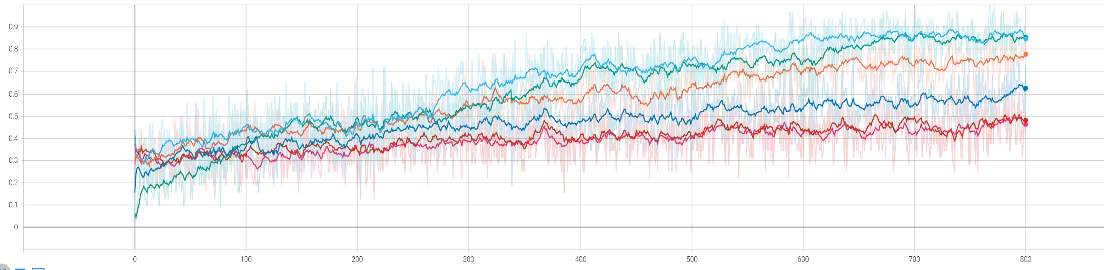
\includegraphics[width=\linewidth]{assets/QA_diagram.pdf}
    \caption{Overview of different hyper parameters  vs Accuracy on test set}
\end{figure}

After selecting our final parameters we achived a final accuracy of 57.66\%, which we validated using a k-fold cross validation strategy

\begin{table*}
\centering
\begin{tabular}{ccc}
\hline \textbf{Model} & \textbf{Plausibility Accuracy} & \textbf{Breakpoint Accuracy} \\ \hline
Baseline & 51.92\% & 48.08\% \\
roberta.large & 56.73\% & 48.08\% \\
roberta.large.mlni & 82.69\% & 60.58\% \\
\hline
\end{tabular}
\caption{\label{font-table} We compare our base model performance to the default roBERTa model on the EAT task and a baseline which always predicts the same class. Only the classification head is optimized and these base models are kept frozen during training.}
\end{table*}

\subsection{Conversational Entailment}

In finding our best model we broke up the process into a few steps. First we tried to overfit the models to essentially memorize the data just to make sure our pipeline was complete and we had a trainable model. Once we did this we experimented with different hyper parameters(optimizer and learning rate) using a grid search.We found that Adam and AdamW did the best with the near default learning rate of 1e-5.We found that this relatively low learning rate made sense as we were just fine tuning the head and using the attention weights that were already pretrained. 

For Epochs and batch size we had an issue that made training a bit more difficult. Our model contained ~330M parameters and doing a forward pass for a single example was a computation and memory heavy operation.We found that we were only able to maintain a batch size of about 5 on the Google Colab GPUs we gained access to, before having memory allocation errors. This also affected the number of epochs the model trained for, since more batch steps means more gradient updates. To figure out how many epochs to run our model we watched convergence behavior during the validation testing and noticed that by epoch 5 the model had shown convergence behavior in all cases. We started by testing on 15 epochs, but changing to 5 significantly cut down further testing time. 

 For The conversational entailment data set we acquired an accuracy of 67.0\% using a 5-fold cross validation strategy. This validation strategy was extremely important since we had such a small data set. The process involved taking all the training data, and first randomizing the order. This was necessary because the data was sorted by entailment.If we didn't randomize we would have buckets with all 1s or 0s, and our model could be seeming to do very well by just predicting always true or false.We then trained our 5 independent models, each time leaving out a bucket of data, then using that bucket as as validation set. We then computed our average validation accuracy over all the models and got our final accuracy of 67.0 percent.

\subsection{EAT}

\begin{figure}[t]
    \centering
    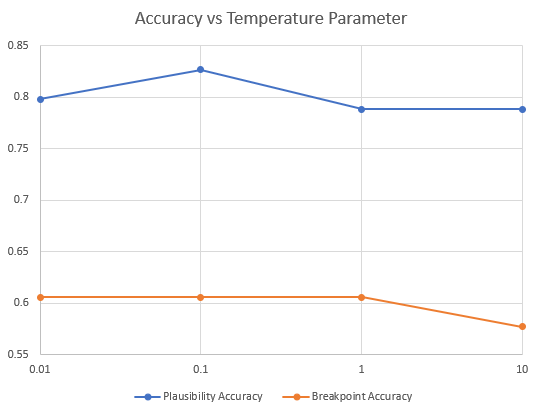
\includegraphics[width=\linewidth]{assets/eat_graph1.png}
    \caption{A comparison of model performance at different temperature parameter settings.}
\end{figure}

For the EAT dataset we performed two main experiments. We first analyzed the impact of utilizing the roBERTa model finetuned on MNLI and then experiment with the temperature parameters. Finally we report the best results of our best model. For speed and efficiency reasons we keep the base network frozen during our experiments and only train the classification head. Additionally, we validate on a random 10\% split of the training data which is held out during training.

For the base model experiment, we compare the roBERTa large model finetuned on MNLI with the regular roBERTa large model. We also include a most common class baseline which always predicts the most common class. Looking at Table 1, we can see that the model finetuned on MLNI significantly outperforms the regular one. In fact, the regular roBERTa large model is only slightly better than the baseline. We suspect this is because the sentence pair embeddings created by the roBERTa model are not particularly meaningful for our contradiction prediction. The finetuning on MLNI, which modifies the base parameters, produces embeddings that are much more aligned with the contradiction prediction task. This also suggests that there could be big performance improvements from unfreezing the base parameters, which we will do later.

We then experimented with different temperature parameters for the smooth maximum function. For each temperature setting we finetune a new classification head on the roBERTa large MNLI base model. Like before, the base model is kept frozen. The results of this experiment can be seen in Figure 3. The accuracy for both tasks does not vary too much between different temperature settings, however it does appear that a maximum is achieved when the temperature parameter is 0.1. This is the setting we use for our best model.

Given the prior experiments, it appears that there is a significant potential for performance improvement if we unfreeze the base model. Using the optimal temperature parameter and base model from before, we take our best checkpoint and perform further finetuning with all parameters unfozen. We found that a smaller learning rate, 2e-6, was necessary to avoid numerical instability and the optimal classification threshold decreased to 0.18. The highest validation accuracy we achieved for the plausibility task was 89.42\%, a breakpoint recall of 30.31\%, a breakpoint precision of 24.11\%, and a f1 score of 73.08\%. Unfortunately we were unable to finish training this model before the competition deadline, so these numbers do not reflect the competition submission, which was our best model with the frozen base. If these numbers are accurate, we think our model is competitive with others in the class. It also seems like the recall and precision are low, which we suspect is due to the class imbalance of the dataset and the relatively small validation set that we use. Some classes might have few or no examples which could bring the average down in a macro average setting.

\section{Discussion}
The first step of any data science project is to scrutinize the data. Some research has pointed to hidden biases of the dataset. Recently, \citet{rajani2019explain} has pointed out “in CQA we observed significant gender disparity and bias with higher proportion of female pronouns used in negative contexts.” For instance, the following are some such examples from CQA:
 
Q: "She was a horrible pet owner, she put a what on her cat?"
AC: wool sweater, get wet, eat vegetables
 
Q: "The woman was yelling obscenities in public,and while it was entertaining for people passing by,what did her husband feel?"
AC: fulfillment, fatigue, embarrassment
 
In other words, it’s reasonable to assume that due to the bias in the training data, the model is more likely to give negative answers or make negative decisions when the subjects are women. This can have significant socioeconomic impact upon the deployment of the model. Recently there have been new methods to prevent biases in data and training, this could be an area of future research.
 
Since we are only reporting on the validation accuracy. We had to split the combined training and validation data into three chucks to include a testing dataset to prevent overfitting to the validation data. (However, the competition in the class uses the full original validation data, providing an incentive for us to not to do a three-way (or cross-validation) and overfit the validation data. With that explicit understanding, the code we provide for the competition will strictly be based on this special circumstance of the competition.) In fact, the test accuracy on the test dataset has a 3 percent drop compared to that on the validation dataset. The fine-grained hyperparameter tuning has made our model slightly overfit the validation dataset. We believe the usage of ensembling, training and tuning several such models independently could help alleviate the problem.
 
We have not used concept net to eliminate potential wrong answer choices, as we know each answer set is 3 concepts from the concept net and 2 are human-created. We rationalize that in real life, we will not know exactly how our data are generated.
 
This research with CommonsenseQA has given us tremendous insights. First, hyperparameter searching and tuning is extremely time-consuming and costly. For natural language processing, one big problem is sequence length. It has a linear relationship with respect to the complexity many of the current state-of-the-art models. When we set the max sequence length to be 80, an ideal choice for our data set, often our platform Google Colab would barely allow us to conduct training. In our experiments with extremely small parameters such as batch size, we have seen similar performance between BERT-large-uncased (0.579248 percent on our validation data set) and BERT-base-uncased. Thus, we performed the fine tuning on BERT-base-uncased.

For the conversational entailment tasks we gained 2 main insights. Firstly, we learned the power of attention based models. For our task it appeared that a statistical model or RNN could be the best solution due to the fact that the task was heavily sequence dependent(with variable length input), but it turned out that attention was the best way to tackle the problem. With attention we  also learned the importance of pretraining and fine tuning. our best model was pretrained on the MNLI task and only the classification head was fine tuned, making my base roBERTa model a very effective encoder. Secondly, we learned a lot about the problems in dealing with small data sets. Because the dataset was small we ran into 2 specific issues: training an effective model, and validating my model. The first part was in training, we believe the reason this task has a relatively low SOTA is due to the small dataset,which made training tricky since getting above a slight chance doesn't always mean our model was going to do well overall. And validating our performance was also difficult since if we test on a set with all false entailment and my model just learns to predict false it will appear that our model is doing much better than it is. This helped me understand validation strategies mentioned more in depth in previous sections.  

In addition, for the conversational entailment task the model we were using was relatively large(330M parameters) and doing forward passes in batches was significantly limited by memory. In most cases a batch size of more than 6 data points was enough to cause a memory allocation problem, this significantly increased our training time as we had to work with very small batch sizes, in addition this also slowed down inference time as we could not vectorize that process. 


One of the biggest lessons we learned from the EAT task was how problem specific a base model's embeddings can be. The act of finetuning on one more dataset changes the output embeddings from being almost useless to very valuable for breakpoint prediction. Through developing our custom loss function we also learned a technique for making the most out of labels that might not encode all the detail that you want. Lastly, we realized the importance of utilizing existing implementations for models and data processing/tokenizing. With the large models that we worked with, experiments take a while to run and thus small bugs can lead to huge amounts of time being wasted. Also with increased complexity there is a greater chance of mistakes, so using established and well tested existing implementations is critical.

\bibliography{acl2020}
\bibliographystyle{acl_natbib}

\appendix

\end{document}
